
\fancyhead[C]{Section 12.6}
\fancyhead[R]{\dayfour}

\section*{\centering Chapter 12.6: Quadric Surfaces}
\textbf{G4: Surfaces.} I can identify standard quadric surfaces including: spheres, ellipsoids, elliptic paraboloids, hyperboloids, cones, and hyperbolic paraboloids. I can match graphs of functions of two variables to their equations and contour plots and determine their domains and ranges.

\subsection*{Mechanics}
\begin{enumerate}
    \item \question{Identify the type of surface described by each of the following. Then roughly sketch each surface, and label one or two key features (eg., if it is a hyperboloid of one sheet, label the "tightest" circle).
	
	\begin{enumerate}
		\item $x^2+4z^2=16$.
		
		\item $9x^2+z^2+y^2=9$.
		
		\item $y^2=3x^2+3z^2$.
		
		\item $z=x^2+y^2+4$.
		
		\item $x^2+y^2=16-z^2$
	\end{enumerate}}

    {% answer goes here

    }
    {% solution goes here
    } 
    \item \question{Consider the family of quadric surfaces $z^2+t = x^2+y^2$, where $t$ is some parameter. What surface type do you get when $t>0$? $t<0$? And when $t =0?$. \\\\
    Check your work with a 3D graphing software of your choice to plot this family, using a "slider" to smoothly vary the parameter $t$ from $-2$ to $2$. As you increase $t$, explain qualitatively what happens near the origin. Where might you witness such a phenomenon in real life?}

    {% answer goes here
    
    }
    {When $t = 0 $, we get a cone. To see this, consider the $z$-cross sections. They exist for all $z\in \R$, and when $z=0$, it is a point, while for all other $z$, they are expanding circles. The only surface which does this is a cone. When $t>0$, observe also that all cross sections exist as well. The difference is that this time, all cross sections are circles (ie., no singular points). This is therefore a hyperboloid of one sheet. Finally, when $t <0$, note that cross sections do not exist whenever $-\sqrt{-t}< z <\sqrt{-t}$, and all other cross sections are circles/points. It follows that we have a hyperboloid of two sheets. \\\\
Qualitatively, as we vary $t$ from the negative numbers to the positive numbers, the two sheets of the hyperboloid come together, and merge into one sheet. This resembles how water droplets when you move them close to each other, and they merge due to water tension. 
    } 
\end{enumerate}
\subsection*{Applications}
\begin{enumerate}[resume]
    \item \question{Quadric surfaces are seen extensively in nature, design and engineering, owing in part to their symmetry. Spot the quadric surfaces in the pictures below, then provide realistic equations for each, including units. 
    }
    {% answer goes here
    
    }
    {% solution goes here
    } 
    
\end{enumerate}
\begin{minipage}{.25\textwidth}
  \centering
  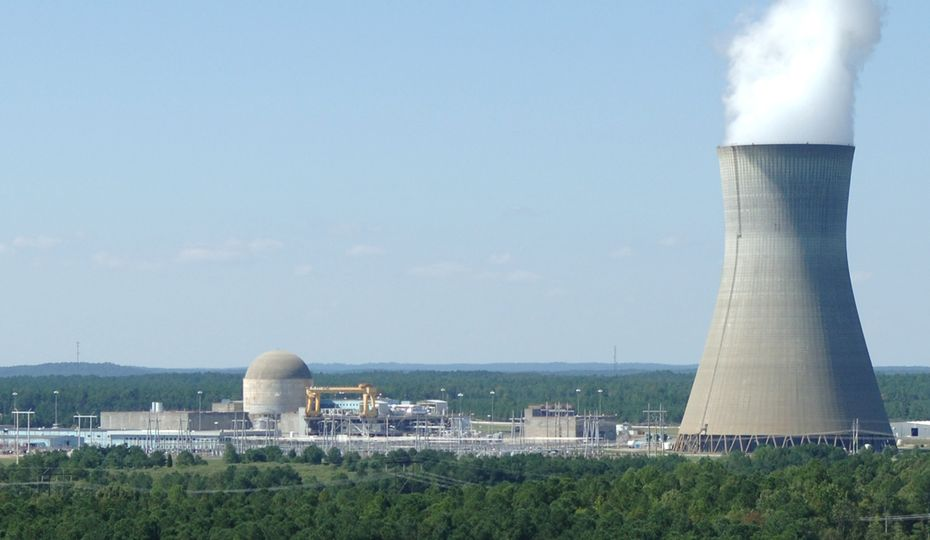
\includegraphics[width=.9\linewidth]{quadric 1.jpg}
\end{minipage}%
\begin{minipage}{.25\textwidth}
  \centering
  
\includegraphics[width=.9\linewidth]{quadric 2.jpg}
\end{minipage}
\begin{minipage}{.25\textwidth}
  \centering
  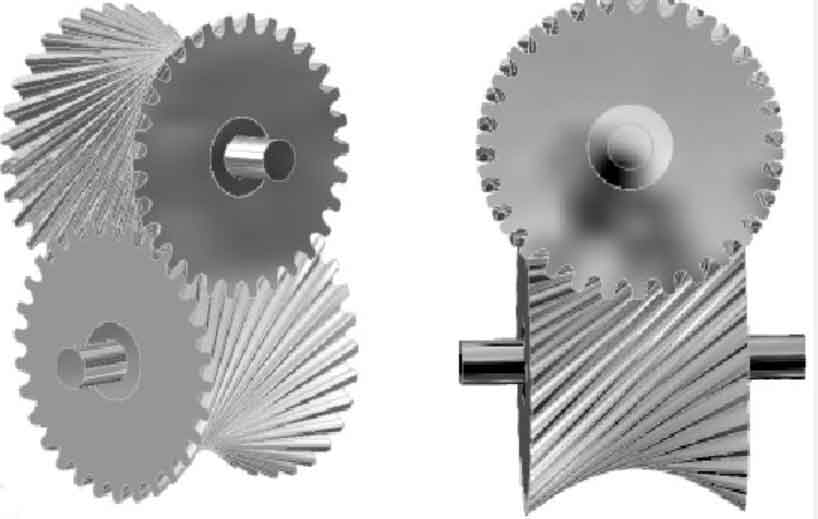
\includegraphics[width=.9\linewidth]{quadric 3.jpg}
\end{minipage}
\begin{minipage}{.25\textwidth}
  \centering
  
\includegraphics[width=.9\linewidth]{quadric 5.jpg}
\end{minipage}

\pagebreak

\subsection*{Extensions}
\begin{enumerate}[resume]
 \item \question{What surface is defined by the equation $x^2 + x -y ^2-y = z^2+z$? }

    {% answer goes here
    }
    {% solution goes here
    } 
 \item \question{Many surfaces arising naturally are \textit{not} quadric, yet the ideas we use to identify quadric surfaces can still be used to deduce their geometry. For example, a surface of extreme importance in statistics is given by $z = e^{-(x^2+y^2)}$. Explain why is this surface not quadric. Then, use the $z$-cross sections to sketch the surface.}

    {% answer goes here
    }
    {% solution goes here
    } 
\end{enumerate}
{}

\iftoggle{answers}{
\fancyhead[R]{\dayfour}
\begin{center}{\large \textbf{Math 2551 Worksheet Answers: Quadric Surfaces}}
\end{center}


\begin{enumerate}
	\item 	
	\begin{enumerate}
		\item elliptical cylinder, oriented along the $y$-axis, cross-sections are ellipses in the $y=k$ planes or vertical/horizontal lines in the $x=k$ and $z=k$ planes.
		
		\item ellipsoid, centered at the origin, wider in the $z$ and $y$ directions than the $x$ direction, cross-sections are circles in the $x=k$ planes (if $k<1$), ellipses in the $z=k$ and $y=k$ planes ($k<3$)
		
		\item circular cone, oriented along the $y$-axis, cross sections are circles in the $y=k$ planes and lines in the $x=k$ and $z=k$ planes
		
		\item elliptical paraboloid, oriented in the positive $z$ direction, shifted up $4$ units, cross-sections are circles in the $z=k$ planes for $k\geq 4$ and parabolas in the $x=k$ or $y=k$ planes
		
		\item sphere, centered at $(0,0,0)$, radius $4$, cross-sections are circles in $x=k, y=k,$ and $z=k$ planes for $0\leq k\leq 4$.
		
	\end{enumerate}
\end{enumerate}
}{}
\iftoggle{solutions}
{
Solutions go here in the same format.
}{}
